\documentclass[
	aspectratio=169, % default is 43
	8pt, % font size, default is 11pt
	%handout, % handout mode without animations, comment out to add animations
	%nosectionframes, % disable automatic frames at the begin of each section (default: sectiontitleslides in beamer mode and sectionoverviews in handout mode)
	%sectiontitleslides, % enable an automatic section title slide at the begin of each section
	%sectionoverviews, % enable an automatic section overview at the begin of each section
]{beamer}

\usepackage{../beamerthemeuulm} % use the inofficial uulm beamer theme
\usepackage{tikz}
\usepackage{amsmath,amssymb}
\usepackage{xcolor}

\usepackage[ruled,linesnumbered]{algorithm2e}
\usepackage{pifont}% http://ctan.org/pkg/pifont
\newcommand{\cmark}{\ding{51}}%
\newcommand{\xmark}{\ding{55}}%
\usepackage{amsmath}
\usepackage{amsfonts}
\usepackage{amssymb}
\usepackage{tikz-qtree}
\usepackage{pgfplotstable}
\usepackage{forest}

\pgfplotsset{
   compat=1.16
}



\newcommand{\VarName}[1]{\textnormal{\emph{#1}}}
\usetikzlibrary{decorations.pathreplacing,calligraphy}
\setfaculty{infIngPsy} % set the color scheme for your faculty here [med/infIngPsy/math/nat]
\usetikzlibrary{positioning}
\usetikzlibrary{overlay-beamer-styles}
\usetikzlibrary{arrows.meta}
\usetikzlibrary{chains,shapes.symbols}
\usetikzlibrary{trees}
\usetikzlibrary{calc}


% Needs
% \usetikzlibrary{calc}
% \usepackage{ifthen}

\def\rotateclockwise#1{
  % Rotate input point by 90 degrees clockwise.
  \newdimen\xrw
  \pgfextractx{\xrw}{#1}
  \newdimen\yrw
  \pgfextracty{\yrw}{#1}
  % \pgfpoint{-\y}{\x}
  \pgfpoint{\yrw}{-\xrw}
}

\def\rotatecounterclockwise#1{
  % Rotate input point by 90 degrees clockwise.
  \newdimen\xrcw
  \pgfextractx{\xrcw}{#1}
  \newdimen\yrcw
  \pgfextracty{\yrcw}{#1}
  % \pgfpoint{-\y}{\x}
  \pgfpoint{-\yrcw}{\xrcw}
}

\def\outsidespacerpgfclockwise#1#2#3{
  % #1 start point
  % #2 end point
  % #3 radius
  % Compute a length-radius vector perpendicular (clockwise)
  % to the vector from start point to end point.
  \pgfpointscale{#3}{
    \rotateclockwise{
      \pgfpointnormalised{
        \pgfpointdiff{#1}{#2}}}}
}

\def\outsidespacerpgfcounterclockwise#1#2#3{
  % #1 start point
  % #2 end point
  % #3 radius
  % Compute a length-radius vector perpendicular (counterclockwise)
  % to the line from start point to end point.
  \pgfpointscale{#3}{
    \rotatecounterclockwise{
      \pgfpointnormalised{
        \pgfpointdiff{#1}{#2}}}}
}

\def\outsidepgfclockwise#1#2#3{
  % #1 start point
  % #2 end point
  % #3 radius
  % Add to end point a length-radius vector perpendicular
  % (counter-clockwise) to the line from start point to end point.
  \pgfpointadd{#2}{\outsidespacerpgfclockwise{#1}{#2}{#3}}
}

\def\outsidepgfcounterclockwise#1#2#3{
  % #1 start point
  % #2 end point
  % #3 radius
  % Add to end point a length-radius vector perpendicular
  % (counter-clockwise) to the line from start point to end point.
  \pgfpointadd{#2}{\outsidespacerpgfcounterclockwise{#1}{#2}{#3}}
}

\def\outside#1#2#3{
  ($ (#2) ! #3 ! -90 : (#1) $)
}

\def\cornerpgf#1#2#3#4{
  % #1 = previous pgf point 
  % #2 = current pgf point
  % #3 = next pgf point
  % #4 = radius
  % Computes a path comprising a rounded corner on the outside of the angle #1#2#3.
  \pgfextra{
    \pgfmathanglebetweenpoints{#2}{\outsidepgfcounterclockwise{#1}{#2}{#4}}
    \let\anglea\pgfmathresult
    \let\startangle\pgfmathresult

    \pgfmathanglebetweenpoints{#2}{\outsidepgfclockwise{#3}{#2}{#4}}
    \pgfmathparse{\pgfmathresult - \anglea}
    \pgfmathroundto{\pgfmathresult}
    \let\arcangle\pgfmathresult
    \ifthenelse{180=\arcangle \or 180<\arcangle}{
      \pgfmathparse{-360 + \arcangle}}{
      \pgfmathparse{\arcangle}}
    \let\deltaangle\pgfmathresult

    \newdimen\x
    \pgfextractx{\x}{\outsidepgfcounterclockwise{#1}{#2}{#4}}
    \newdimen\y
    \pgfextracty{\y}{\outsidepgfcounterclockwise{#1}{#2}{#4}}
  }
  -- (\x,\y) arc [start angle=\startangle, delta angle=\deltaangle, radius=#4]
}

\def\corner#1#2#3#4{
  \cornerpgf{\pgfpointanchor{#1}{center}}{\pgfpointanchor{#2}{center}}{\pgfpointanchor{#3}{center}}{#4}
}

\def\hedgeiii#1#2#3#4{
  % #1#2#3 = tikz points
  % #4 = radius
  % Computes a path comprising the line of the points outside of the
  % convex hull H of the points #1#2#3 that have distance #4 to H.
  % Points #1#2#3 need to be in clockwise order.
  \outside{#1}{#2}{#4} \corner{#1}{#2}{#3}{#4} \corner{#2}{#3}{#1}{#4} \corner{#3}{#1}{#2}{#4} -- cycle
}

\def\hedgem#1#2#3#4{
  % #1#2 = tikz points
  % #3 = list of tikz points
  % #4 = radius
  % Computes a path comprising the line of the points outside of the convex hull H of the points #1#2[#3] that have distance #4 to H.
  % Points #1#2[#3] need to be vertices of a convex polygon and in clockwise order.
  
  \outside{#1}{#2}{#4}
  \pgfextra{
    \def\hgnodea{#1}
    \def\hgnodeb{#2}
  }
  foreach \c in {#3} {
    \corner{\hgnodea}{\hgnodeb}{\c}{#4}
    \pgfextra{
      \global\let\hgnodea\hgnodeb
      \global\let\hgnodeb\c
    }
  }
  \corner{\hgnodea}{\hgnodeb}{#1}{#4}
  \corner{\hgnodeb}{#1}{#2}{#4}
  -- cycle
}

\def\hedgeii#1#2#3{
  % #1#2 = tikz points
  % #3 = radius
  \hedgem{#1}{#2}{}{#3}
}

\def\hedgei#1#2{
  % #1 = tikz point
  % #2 = radius
  (#1) circle [radius = #2]
}
\tikzset{hide on/.code={\only<#1>{\color{white}}}}


%\institutelogo{sp} % set the institute logo
%\universitylogo{uulm} % set a new university logo
%\clearuniversitylogo % clear existing university logo
%\clearinstitutelogo % clear existing institute logo
%\uulmlogos{sp,uulm} % freely configure multiple logos (overwrites any other logo setting)

%\usepackage[ngerman]{babel} % use this line for slides in German

%\setmycolumnsdefault{keep} % change the default for 'mycolumns' environment (e.g., 'keep' to animate all column environments per default)

%\includeonlyframes{current} % default mechanism of beamer to include only labeled frames, can be used for debugging or drafting

\title[Projected d-DNNF Compilation]{Projected d-DNNF Compilation for Feature Models} % short title is used for the slide footer but optional
\subtitle{Master's Thesis} % subtitles are optional at all
\author[Jacob Loth]{Jacob Loth} % short author title is used for the slide footer but optional
\date{\today} % use a particular date here if needed

\begin{document}

\maketitle % title page with default picture

\section{Motivation}

\subsection{Feature Models}
\begin{frame}{\insertsubsection}
	\centering
	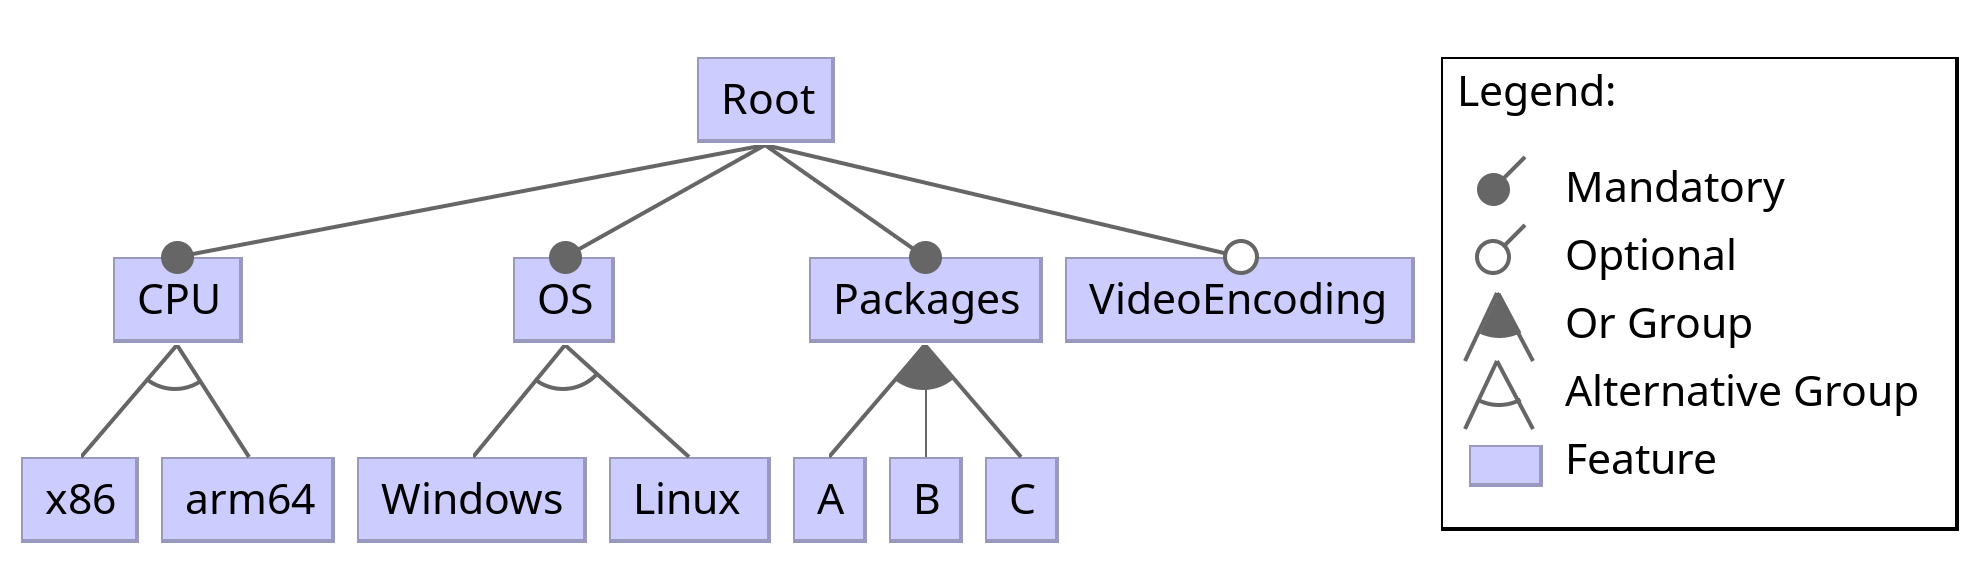
\includegraphics[width=10cm]{fm.png}
    \begin{block}{}
        We can convert feature models to propositional formulas!
        \begin{equation*}
            (\text{x86} \land \neg \text{arm64}) \lor (\neg \text{x86} \land \text{arm64}) ...
        \end{equation*}
    \end{block}
\end{frame}
\subsection{Feature-Model Slicing}
\tikzstyle{tree}=[draw=black,thick,anchor=west]
\tikzstyle{selected}=[draw=red,fill=red!30]
\tikzstyle{optional}=[dashed,fill=gray!50]
\begin{frame}{\insertsubsection}
	\begin{block}{Feature Model}
	\centering
	\begin{tikzpicture}[%
	  grow via three points={one child at (0.5,-0.7) and
	  two children at (0.5,-0.7) and (0.5,-1.4)},
	  edge from parent path={(\tikzparentnode.south) |- (\tikzchildnode.west)}]
	\node[tree](hw) {Hardware}
		child { node[tree] {arm64}}		
		child { node[tree] {x86}}
		child { node[tree] {VideoEncoding}};
	\node[tree](sw)[right = 4cm of hw] {Software}
		child { node[tree] {Windows}}	
		child { node[tree] {Linux}}			
		child { node[tree] {Packages*}};
	\draw[<->, visible on=<2->] (sw) -- (hw) node[midway,fill=white] {\emph{constraints}};
	\end{tikzpicture}
	\end{block}
	\begin{block}<3->{Problem}
		How many hardware configurations?
	\end{block}
	\begin{block}<4->{Transitive Constraints}

		\begin{tabular}[t]{cc}
			$\text{VideoEncoding} \implies \text{Windows}$&\visible<5>{  \hspace{0.5cm}$\text{Sliced: VideoEncoding} \implies \text{x86}$}\\
			$\text{Windows}\implies \text{x86}$ &
		\end{tabular}
	\end{block}
    
\end{frame}
\begin{frame}{Model Counting}
   
    
    \begin{block}{Problem}
    \begin{itemize}
        \item  {\color{red} How many} hardware configurations?\pause
        \item Counting the number of satisfiable assignments of a propositional formula $F$. Denoted as $|F|$.
    \end{itemize}    
    
    \vspace{0.5cm}
    \begin{displaymath}
        \begin{array}{|c c|c|}
        % |c c|c| means that there are three columns in the table and
        % a vertical bar ’|’ will be printed on the left and right borders,
        % and between the second and the third columns.
        % The letter ’c’ means the value will be centered within the column,
        % letter ’l’, left-aligned, and ’r’, right-aligned.
        p & q & F=a \land b\\ % Use & to separate the columns
        \hline % Put a horizontal line between the table header and the rest.
        \color{blue}1 & \color{blue}1 & \color{blue}1\\
        1 & 0 & 0\\
        0 & 1 & 0\\
        0 & 0 & 0\\
        \end{array}
        \end{displaymath}
    
    \end{block}
    \centering\pause
    
\begin{tikzpicture}[]
        \node[draw](sharpsat){\color{magenta} \bf \#SAT};
    \end{tikzpicture}\\
    Counts the number of solutions of a propositional formula. \\
    Worst-case exponential complexity!
    \end{frame}
    \begin{frame}{d-DNNF}
        \begin{columns}[]
            \begin{column}{.5\textwidth}
                Any propositional formula which is:\\
                \begin{block}<1->{{\bf d}eterministic}
                    Exclusive or-operators $F=A \lor B$\\
                    Never simultaneous $A=1$ and $B=1$\\
                    If-then-else\\
                    $|F|=|A|+|B|$\\
                \end{block}
                \begin{block}<3->{{\bf D}ecomposable}
                    And-operands $F=A \land B$ never share variables\\
                    $|F|=|A|*|B|$\\
                \end{block}
                \begin{block}<5->{{\bf N}egation {\bf N}ormal {\bf F}orm}
                \end{block}
            \end{column}
            \begin{column}{.5\textwidth}
                \begin{center}
                    
               
                \only<1-2>{
                \begin{forest}
                    for tree={ s sep+=12pt,
                    l sep+=12pt}
                    [$\lor$
                        [$a \land b$]
                        [$c \land \only<2>{\neg} b$],edge label={node[midway,left,font=\scriptsize]{1}}
                    ] 
                \end{forest}}
                \only<3->{
                    \begin{forest}
                        for tree={ s sep+=12pt,
                        l sep+=12pt}
                        [$\land$
                            [$a\lor b$]
                            [${\color{red}\only<3>{b}}{\color{green}\only<4->{d}}\lor c$],edge label={node[midway,left,font=\scriptsize]{1}}
                        ] 
                    \end{forest}}\\
                \vspace{0.1cm}
                \only<1>{Not a d-DNNF {\color{red} \xmark}}
                \only<2>{A d-DNNF {\color{green} \checkmark}}
                \only<3>{Not a d-DNNF {\color{red} \xmark}}
                \only<4>{A d-DNNF {\color{green} \checkmark}}
            \end{center}
            \end{column}
            
        \end{columns}
        \visible<6->{
        \begin{center}
            {\bf d-DNNF formulas allow linear-time model counting\\
            d-DNNF Compilation: CNF $\rightarrow$ d-DNNF\\
            Knowledge-Compilation: It's still just a formula }}
        \end{center}
    \end{frame}

\begin{frame}{\insertsubsection}
	\begin{block}{Problem}
		\only<1>{{\color{red} How many} hardware configurations?}
		\only<2>{ How many hardware configurations {\color{red} with arm64?}}
		\only<3->{ How many hardware configurations {\color{red} with X ?}}
	\end{block}
	\only<0->{
	\begin{tikzpicture}[]
		\node[tree](fm){Feature-Model};
		\node[tree,right= 0.5cm of fm](cnf){\begin{tabular}{c} CNF: \\ $(A \lor B \lor \neg C) \land (\neg B \lor \neg C) \dots$  \end{tabular}};
		\node[tree,tree,right= 0.5cm of cnf,visible on = <1-6>](slice){\begin{tabular}{c} Slice:\\$(A \lor B)\land (\neg B)\dots$\end{tabular}};
		\node[right= 1.5cm of slice,visible on=<1-3>,draw](sharpsat){\color{magenta} \bf \#SAT };
		\node[below= 0.7cm of sharpsat,visible on=<2-3>,draw](sharpsat1){\color{magenta} \bf \#SAT};
		\node[above= 0.7cm of sharpsat,visible on=<3-3>](sharpsatN){$...$};
		\node[right= 1.0cm of slice,visible on=<4-6>,draw](ddnnf){\color{magenta} \bf \begin{tabular}{c}d-DNNF\\Compilation\end{tabular} };
		\node[above= 0.5cm of ddnnf,visible on=<5-6>,draw=black,thick](queries){\begin{tabular}{l} Counting Queries:\\arm64=true\\ $\dots$ \end{tabular} };
        \node[right= 1.0cm of cnf,visible on=<7>,draw](pmc){\color{magenta} \bf \begin{tabular}{c}Projected\\Model\\Counting\end{tabular}  };
		\node[right= 1.0cm of cnf,visible on=<8>,draw](pddnnf){\color{magenta} \bf \begin{tabular}{c}Projected\\d-DNNF\\Compilation\end{tabular}  };
		\node[above= 0.5cm of pddnnf,visible on=<8>,draw=black,thick](queries1){\begin{tabular}{l} Counting Queries:\\arm64=true\\ $\dots$ \end{tabular} };
		\draw[->] (fm)--(cnf);
		\draw[->,visible on = <1-6>] (cnf)--(slice);
		\draw[->,visible on = <1-3>] (slice)--(sharpsat);
		\draw[->,visible on=<2-3>] (slice.east)--(sharpsat1.west) node[near end,left] {arm64=true};
		\draw[->,visible on=<3-3>] (slice.east)--(sharpsatN.west);
        \draw[->,visible on=<4-6>] (slice.east)--(ddnnf);
		\draw[->,visible on=<5-6>] (queries)--(ddnnf);
        \draw[->,visible on=<7>] (cnf)--(pmc);
		\draw[->,visible on=<8>] (cnf)--(pddnnf);
		\draw[->,visible on=<8>] (queries1)--(pddnnf);
		\draw [decorate,
    decoration = {brace},thick,red,visible on = <6>] (11,-0.75) --  (7.3,-0.75) node[midway,below] {can be slow};
	\end{tikzpicture}}
\end{frame}
\begin{frame}{Slicing Implementation\footnote{Comparing Algorithms for Efficient Feature-Model Slicing, Krieter et al.}}
    Resolve all clauses with $v$ with all clauses with $\neg v$
    \begin{block}<1->{Resolving Two Clauses}
        \begin{equation*}
            \begin{split}
            (\neg VideoEncoding \lor Windows), (x86 \lor \neg Windows) &\rightarrow (\neg VideoEncoding \lor x86)\\
            \visible<2->{ (a_1 \lor a_2 \lor  ...  \lor v), (b_1 \lor b_2 \lor  ... \lor \neg v) & \rightarrow (a_1 \lor a_2 \lor  ... \lor b_1 \lor b_2 \lor ...)}
           % (VideoEncoding \implies Windows), (x86 \implies Windows) &\rightarrow (VideoEncoding  \implies x86)\\
            \end{split}
        \end{equation*}
    \end{block}
    \begin{block}<3->{Resolving Many Clauses}
        \begin{center}
        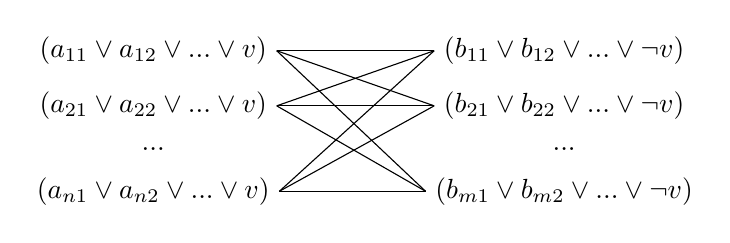
\begin{tikzpicture}
            \node (l1) {$(a_{11} \lor a_{12} \lor ... \lor v)$};
            \node[below = 0.1cm of l1] (l2) {$(a_{21} \lor a_{22} \lor ... \lor v)$};
            \node[below = 0.1cm of l2] (l3) {$...$};
            \node[below = 0.1cm of l3] (l4) {$(a_{n1} \lor a_{n2} \lor ... \lor v)$};
            \node[right = 2cm of l1] (r1) {$(b_{11} \lor b_{12} \lor ... \lor \neg v)$};
            \node[below = 0.1cm of r1] (r2) {$(b_{21} \lor b_{22} \lor ... \lor \neg v)$};
            \node[below = 0.1cm of r2] (r3) {$...$};
            \node[below = 0.1cm of r3] (r4) {$(b_{m1} \lor b_{m2} \lor ... \lor \neg v)$};
            \path[draw] (l1.east) -- (r1.west);
            \path[draw] (l1.east) -- (r2.west);
            \path[draw] (l1.east) -- (r4.west);
            \path[draw] (l2.east) -- (r1.west);
            \path[draw] (l2.east) -- (r2.west);
            \path[draw] (l2.east) -- (r4.west);
            \path[draw] (l4.east) -- (r1.west);
            \path[draw] (l4.east) -- (r2.west);
            \path[draw] (l4.east) -- (r4.west);
        \end{tikzpicture}\\
        \visible<3->{
        \vspace{0.1cm}
        {\bf Exponential clause count increase for multiple variables.}\\
        }
    \end{center}
    \end{block}
    
    
\end{frame}





\subsection{d-DNNF Compilation}

\begin{frame}{\insertsubsection}
	\begin{columns}[c]
		\begin{column}{.5\textwidth}
	\centering
	\begin{block}{DPLL}
	\begin{overlayarea}{10cm}{4.44cm}
		

		

	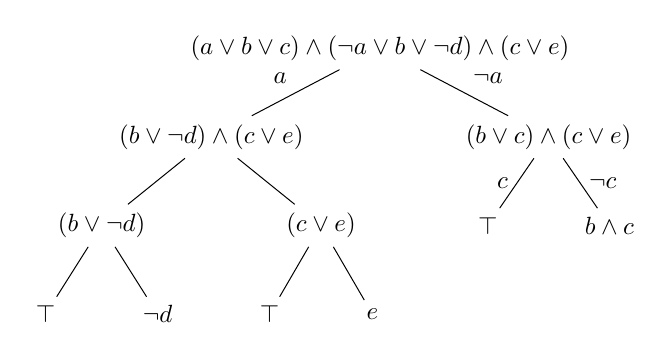
\begin{tikzpicture}[every tree node/.style={},
	level distance=1.25cm,sibling distance=1cm,
	scale=0.9,
	edge from parent path={(\tikzparentnode) -- (\tikzchildnode)}]
 \Tree
 [. \node[visible on=<1->]{$(a \lor b \lor c) \land (\neg a \lor b  \lor \neg d ) \land (c \lor e)$};
	 \edge[visible on=<2->] node[auto=right] {$a$};
	 [. \node[visible on=<2->]{$( b  \lor \neg d ) \land (c \lor e)$ };
	 	\edge[visible on=<4->] node[auto=right] {$$};
	 	[. \node[visible on=<4->]{$(b \lor \neg d)$} ;
		 	\edge[visible on=<5->] node[auto=right] {$$};
	 		[.\node[visible on=<5->] {$\top$};  ] 
			\edge[visible on=<5->] node[auto=right] {$$};
	 		[.\node[visible on=<5->]{$\neg d$};  ] 
	 	]
		\edge[visible on=<4->] node[auto=right] {$$};
	 	[.\node[visible on=<4->]{$(c \lor e)$};
		 	\edge[visible on=<6->] node[auto=right] {$$};
	 		[.\node[visible on=<6->]{$\top$};  ]
			 \edge[visible on=<6->] node[auto=right] {$$};
			[.\node[visible on=<6->]{$e$};  ] 
	]
	]
	 \edge[visible on=<3->] node[auto=left] {$\neg a$};
	 [.\node[visible on=<3->]{$(b \lor c) \land (c \lor e)$};
		 \edge[visible on=<7->] node[midway,left] {$c$};
		 [.\node[visible on=<7->]{$\top$};  ]
		 \edge[visible on=<7->] node[midway,right] {$\neg c$};
		 [.\node[visible on=<7->]{$b \land c$};  ]
	]
 ]
 \end{tikzpicture}
\end{overlayarea}


\end{block}
\end{column}
\begin{column}{.5\textwidth}
	\begin{block}<8>{d-DNNF}
		
	\centering
	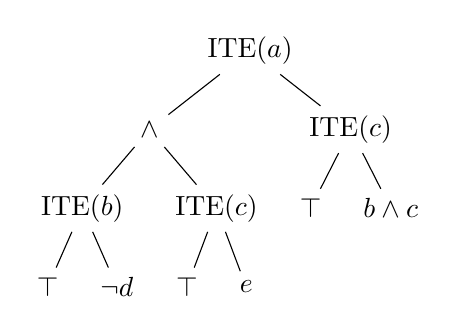
\begin{tikzpicture}[every tree node/.style={},
		level distance=1cm,sibling distance=0.3cm,
		scale=1.,
		edge from parent path={(\tikzparentnode) -- (\tikzchildnode)}]
	 \Tree
	 [.{$\text{ITE}(a)$}
		 [.{$\land$ }
		 [.{$\text{ITE}(b)$}  
		 [.{$\top$}  ] 
		 [.{$\neg d$}  ] 
		 ]
		 [.{$\text{ITE}(c)$}  
			 [.{$\top$}  ] 
			[.{$e$}  ] 
		]
		]
		 [.{$\text{ITE}(c)$} 
			 [.{$\top$}  ]
			 [.{$b \land c$}  ]
		]
	 ]
	 \end{tikzpicture}
	
	\end{block}
	\begin{block}<8>{}
		\hspace{1cm} ITE = If Then Else
	\end{block}

	

\end{column}
\end{columns}
\end{frame}
\begin{frame}{Heuristics}
    Vanilla DPLL is very slow
    \begin{block}<2->{Variable Odering}
        \begin{center}
            \only<1-2>{
            \visible<2>{
            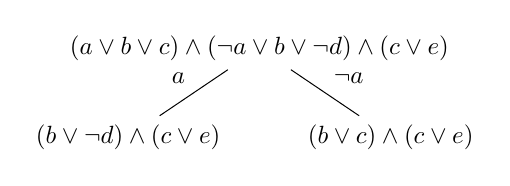
\begin{tikzpicture}[every tree node/.style={},
                level distance=1.25cm,sibling distance=1cm,
                scale=0.9,
                edge from parent path={(\tikzparentnode) -- (\tikzchildnode)}]
             \Tree
             [. \node[]{$(a \lor b \lor c) \land (\neg a \lor b  \lor \neg d ) \land (c \lor e)$};
                 \edge[] node[auto=right] {$a$};
                [. \node[]{$( b  \lor \neg d ) \land (c \lor e)$ };]
                \edge[] node[auto=left] {$\neg a$};
                [.\node[]{$(b \lor c) \land (c \lor e)$};]
             ]
             \end{tikzpicture}}}
             \only<3>{
             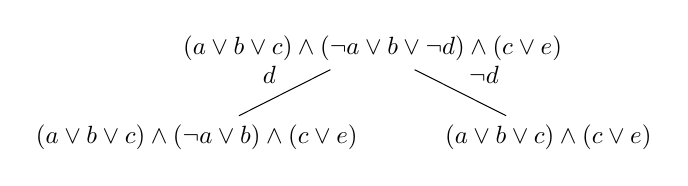
\begin{tikzpicture}[every tree node/.style={},
                level distance=1.25cm,sibling distance=1cm,
                scale=0.9,
                edge from parent path={(\tikzparentnode) -- (\tikzchildnode)}]
             \Tree
             [. \node[]{$(a \lor b \lor c) \land (\neg a \lor b  \lor \neg d ) \land (c \lor e)$};
                 \edge[] node[auto=right] {$d$};
                [. \node[]{$(a \lor b  \lor  c ) \land (\neg a \lor b) \land (c \lor e)$ };]
                \edge[] node[auto=left] {$\neg d$};
                [.\node[]{$(a \lor b  \lor  c ) \land (c \lor e)$};]
             ]
             \end{tikzpicture}}
            \end{center}
    \end{block}
    
\end{frame}

\begin{frame}{Heuristics: Dual Hypergraph}
    \begin{center}
        

    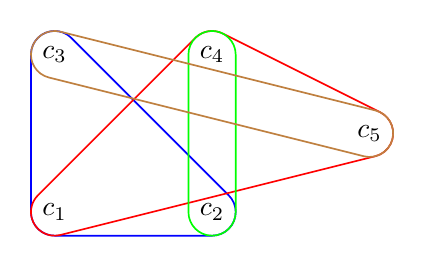
\begin{tikzpicture}
        [
            he/.style={draw, semithick},        % he = hyper edge
            ce/.style={draw,dashed, rounded corners=10pt}, % ce = condition edge
        ]
        \node (a) at (0,0) {$c_1$};
        \node (b) at (2,0) {$c_2$};
        \node (c) at (0,2) {$c_3$};
        \node (d) at (2,2) {$c_4$};
        \node (e) at (4,1) {$c_5$};
        \draw[he,color=blue] \hedgeiii{c}{b}{a}{3mm};
        \draw[he,color=red] \hedgeiii{a}{d}{e}{3mm};
        \draw[he,color=green] \hedgeii{b}{d}{3mm};
        \draw[he,color=brown] \hedgeii{c}{e}{3mm};
        %$\node [ce, fit=(g) (e)] {};
        %\node [fit=(a) (b) (d)] (fd){};%\draw [dashed,rounded corners=10pt] ($(fd.south west)+(0,-0.5)$) -- (fd.north west) -- ($(fd.north east)+(0.5,0)$)--cycle;
        \end{tikzpicture}
        \visible<2->{
        \hspace{1cm}
            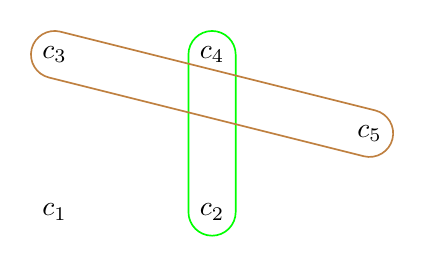
\begin{tikzpicture}
                [
                    he/.style={draw, semithick},        % he = hyper edge
                    ce/.style={draw,dashed, rounded corners=10pt}, % ce = condition edge
                ]
                \node (a) at (0,0) {$c_1$};
                \node (b) at (2,0) {$c_2$};
                \node (c) at (0,2) {$c_3$};
                \node (d) at (2,2) {$c_4$};
                \node (e) at (4,1) {$c_5$};
                \draw[he,color=green] \hedgeii{b}{d}{3mm};
                \draw[he,color=brown] \hedgeii{c}{e}{3mm};
                %$\node [ce, fit=(g) (e)] {};
                %\node [fit=(a) (b) (d)] (fd){};%\draw [dashed,rounded corners=10pt] ($(fd.south west)+(0,-0.5)$) -- (fd.north west) -- ($(fd.north east)+(0.5,0)$)--cycle;
                \end{tikzpicture}}
   
        \end{center}
        \begin{block}{Construction}
            $F=\underset{c_1}{({\color{blue}a} \lor {\color{red}b})} \land \underset{c_2}{({\color{blue}a} \lor \neg {\color{green}c})} \land \underset{c_3}{({\color{blue}a} \lor \neg {\color{brown}d})} \land 
            \underset{c_4}{({\color{red}b} \lor \neg {\color{green}c})}\land \underset{c_5}{( {\color{red}b} \lor \neg {\color{brown}d})}$\\
            \vspace{0.1cm}
            \begin{center}
                \bf Split formula into independent sub-problems of roughly equal size.\\
            \end{center}
        \end{block}
         
\end{frame}
\section{Our Contributions}

\begin{frame}[fragile]{Projected d-DNNF Compilation}
	\begin{block}{Concept}
	Projected variables = $a,b,d$\\
	Sliced variables = $c,e$
	\end{block}
	
	\begin{block}{}
		\centering
		\begin{overlayarea}{10cm}{4.44cm}
\begin{tikzpicture}[every tree node/.style={},
	level distance=1.25cm,sibling distance=1cm,
	scale=0.9,
	edge from parent path={(\tikzparentnode) -- (\tikzchildnode)}]
 \Tree
 [. \node[visible on=<1->]{$(a \lor b \lor c) \land (\neg a \lor b  \lor \neg d ) \land (c \lor e)$};
	 \edge[visible on=<2->] node[auto=right] {$a$};
	 [. \node[visible on=<2->]{$( b  \lor \neg d ) \land (c \lor e)$ };
	 	\edge[visible on=<4->] node[auto=right] {$$};
	 	[. \node[visible on=<4->]{$(b \lor \neg d)$} ;
		 	\edge[visible on=<5->] node[auto=right] {$$};
	 		[.\node[visible on=<5->] {$\top$};  ] 
			\edge[visible on=<5->] node[auto=right] {$$};
	 		[.\node[visible on=<5->]{$\neg d$};  ] 
	 	]
		\edge[visible on=<4->] node[auto=right] {$$};
	 	[.\node[visible on=<4->]{\only<4-5>{$(c \lor e)$} \only<6->{\color{red} $\top$}  };]
	]
	 \edge[visible on=<3->] node[auto=left] {$\neg a$};
	 [.\node[visible on=<3->]{$(b \lor c) \land (c \lor e)$};
		 \edge[visible on=<7->] node[midway,left] {$b$};
		 [.\node[visible on=<7->]{$\top$};  ]
		 \edge[visible on=<7->] node[midway,right] {$\neg b$};
		 [.\node[visible on=<7->]{  \only<7>{ $(c \lor e)$ } \only<8->{\color{red} $\top$}   };  ]
	]
 ]
 \end{tikzpicture}
\end{overlayarea}
\end{block}
\end{frame}
\begin{frame}{Integration and Optimization in D4\footnote{An Improved Decision-DNNF Compiler, Lagniez et al.}}
    \begin{center}
        
    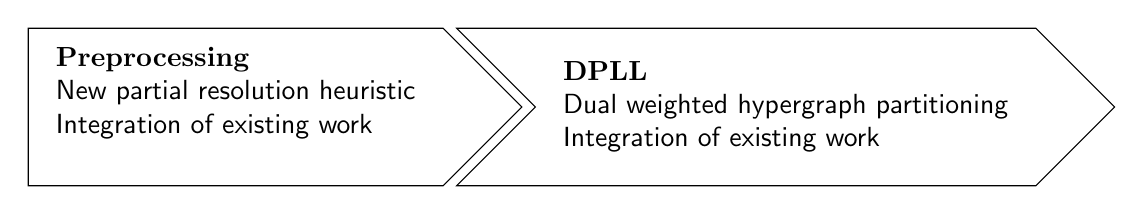
\begin{tikzpicture}[nodes={shape=signal,signal from=west, signal to=east,
        align=left,font=\sffamily,draw,on chain,minimum height=2cm,
        inner xsep=1em},start chain=going right,node distance=1ex]
     \path node[signal from=nowhere]{{\bf Preprocessing}\\New partial resolution heuristic\\Integration of existing work\\}   
       node{{\bf DPLL} \\ Dual weighted hypergraph partitioning\\ Integration of existing work };
    \end{tikzpicture}
    \end{center}
\end{frame}
\begin{frame}{Dual Weighted Hypergraph Partitioning}

      \begin{center}
        
  
        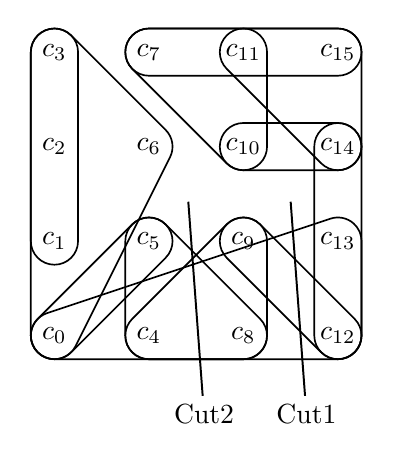
\begin{tikzpicture}
            [
                he/.style={draw, semithick},        % he = hyper edge
                ce/.style={draw,dashed, rounded corners=10pt}, % ce = condition edge
            ]
            \node []  (00) at (1.2*0,1.2*0) {$c_0$};
            \node []  (01) at (1.2*0,1.2*1) {$c_1$};
            \node []  (02) at (1.2*0,1.2*2) {$c_2$};
            \node []  (03) at (1.2*0,1.2*3) {$c_3$};
            \node []  (10) at (1.2*1,1.2*0) {$c_4$};
            \node []  (11) at (1.2*1,1.2*1) {$c_5$};
            \node []  (12) at (1.2*1,1.2*2) {$c_6$};
            \node []  (13) at (1.2*1,1.2*3) {$c_7$};
            \node []  (20) at (1.2*2,1.2*0) {$c_8$};
            \node []  (21) at (1.2*2,1.2*1) {$c_9$};
            \node []  (22) at (1.2*2,1.2*2) {$c_{10}$};
            \node []  (23) at (1.2*2,1.2*3) {$c_{11}$};
            \node []  (30) at (1.2*3,1.2*0) {$c_{12}$};
            \node []  (31) at (1.2*3,1.2*1) {$c_{13}$};
            \node []  (32) at (1.2*3,1.2*2) {$c_{14}$};
            \node []  (33) at (1.2*3,1.2*3) {$c_{15}$};
            \draw[line width=0.25mm,visible on=<4->] (1.7,1.7)--(1.9,-1)node[at end,fill=white]{ Cut2};
            \draw[line width=0.25mm,visible on=<2->] (3,1.7)--(3.2,-1)node[at end,fill=white]{Cut1};
            \draw[he] \hedgeiii{00}{03}{12}{3mm};
            \draw[he] \hedgeiii{10}{21}{20}{3mm};
            \draw[he] \hedgeiii{00}{31}{30}{3mm};
            \draw[he] \hedgeiii{13}{23}{22}{3mm};
            \draw[he] \hedgeiii{13}{23}{33}{3mm};
            \draw[he] \hedgeii{22}{32}{3mm};
            \draw[he,alt=<{1,2}>{black}{red}] \hedgeiii{01}{02}{03}{3mm};
            \draw[he] \hedgeiii{10}{11}{20}{3mm};
            \draw[he,alt=<{1,2}>{black}{red}] \hedgeiii{32}{23}{33}{3mm};
            \draw[he,alt=<{1,2}>{black}{red}] \hedgeiii{30}{31}{32}{3mm};
            \draw[he,alt=<{1,2}>{black}{red}] \hedgeii{00}{11}{3mm};
            \draw[he,alt=<{1,2}>{black}{red}] \hedgeii{30}{21}{3mm};
          
            %$\node [ce, fit=(g) (e)] {};
            %\node [fit=(a) (b) (d)] (fd){};%\draw [dashed,rounded corners=10pt] ($(fd.south west)+(0,-0.5)$) -- (fd.north west) -- ($(fd.north east)+(0.5,0)$)--cycle;
            \end{tikzpicture}
        \end{center}
        $F=c_0\land c_1 \land ... \land c_{15}$
\end{frame}
\begin{frame}[t]{Partial Resolution}
\vspace{0.5cm}
Greedily resolve "easy" sliced variables until the clause count increases\\
\only<2-4>{
\begin{block}{Clause Ratio}
    

$F=(a \lor b \lor c) \land (\neg a \lor b  \lor \neg d ) \land (c \lor e)$\\
Sliced variables = $c,e$\\
\vspace{0.1cm}
{\bf Resolution of $c$ and $e$ is trivial} $\implies F = (\neg a \lor b  \lor \neg d )$ 
\begin{center}
    
\only<3>{
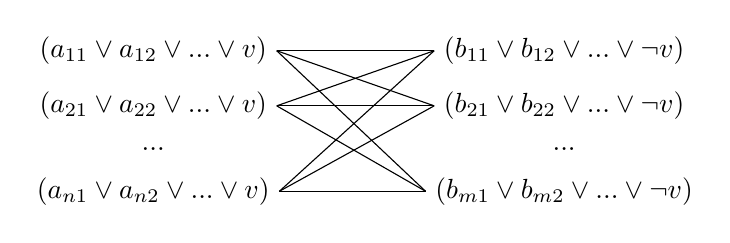
\begin{tikzpicture}
    \node (l1) {$(a_{11} \lor a_{12} \lor ... \lor v)$};
    \node[below = 0.1cm of l1] (l2) {$(a_{21} \lor a_{22} \lor ... \lor v)$};
    \node[below = 0.1cm of l2] (l3) {$...$};
    \node[below = 0.1cm of l3] (l4) {$(a_{n1} \lor a_{n2} \lor ... \lor v)$};
    \node[right = 2cm of l1] (r1) {$(b_{11} \lor b_{12} \lor ... \lor \neg v)$};
    \node[below = 0.1cm of r1] (r2) {$(b_{21} \lor b_{22} \lor ... \lor \neg v)$};
    \node[below = 0.1cm of r2] (r3) {$...$};
    \node[below = 0.1cm of r3] (r4) {$(b_{m1} \lor b_{m2} \lor ... \lor \neg v)$};
    \path[draw] (l1.east) -- (r1.west);
    \path[draw] (l1.east) -- (r2.west);
    \path[draw] (l1.east) -- (r4.west);
    \path[draw] (l2.east) -- (r1.west);
    \path[draw] (l2.east) -- (r2.west);
    \path[draw] (l2.east) -- (r4.west);
    \path[draw] (l4.east) -- (r1.west);
    \path[draw] (l4.east) -- (r2.west);
    \path[draw] (l4.east) -- (r4.west);
\end{tikzpicture}}

\only<4>{
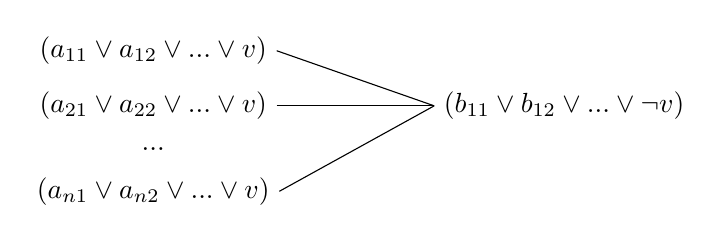
\begin{tikzpicture}
    \node (l1) {$(a_{11} \lor a_{12} \lor ... \lor v)$};
    \node[below = 0.1cm of l1] (l2) {$(a_{21} \lor a_{22} \lor ... \lor v)$};
    \node[below = 0.1cm of l2] (l3) {$...$};
    \node[below = 0.1cm of l3] (l4) {$(a_{n1} \lor a_{n2} \lor ... \lor v)$};
    \node[right = 2cm of l2] (r1) {$(b_{11} \lor b_{12} \lor ... \lor \neg v)$};
    \path[draw] (l1.east) -- (r1.west);
    \path[draw] (l2.east) -- (r1.west);
    \path[draw] (l4.east) -- (r1.west);
\end{tikzpicture}}
\end{center}
\end{block}}

\only<5-7>{
 
\begin{block}{Connectivity}
    $(\neg a \lor b \lor v),(a \lor b \lor \neg v) \rightarrow (\neg a \lor b \lor b \lor c)\equiv \top$\\
    \vspace{0.1cm}
    \visible<6->{{{\bf Simpical Variable~\footnotemark[1]}: neighbors form a clique through clauses}}\\
    \visible<7->{
    \begin{center}

    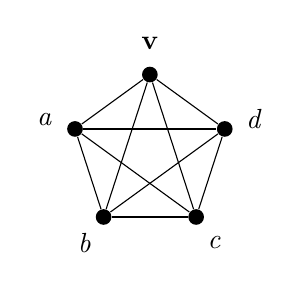
\begin{tikzpicture}[bullet/.style={circle, fill, inner sep=2pt}]
        \foreach \lab [count=\c, 
                       evaluate=\c as \ang using {18+72*\c}] 
        in {{\bf v},{\it a}, {\it b}, {\it c},{\it d}} {
           \node[bullet] (\c) at (\ang:10mm) {};
           \node at (\ang:14mm){$\lab$};
           \foreach \i in {1,...,\c} {
              \draw(\i)--(\c);
           }
        }
      \end{tikzpicture}\\
    \end{center}}

    \only<6->{{\footnotesize \footnotemark[1]from GPMC source code}}

    
\end{block}}

\begin{block}<8->{New Combined Heuristic}
    Group by:
    \begin{enumerate}
        \item Trivial resolution variables
        \item Simpical variables
        \item Other variables
    \end{enumerate}
    Sort by: $v_p*v_n$ and average clause length
    \begin{center}
    \begin{tikzpicture}
        \tikzset{
          bound/.style={
            draw,
            minimum height=2cm,
            inner sep=1em,
          },
          arrow/.style={
            draw,
            minimum height=1cm,
            inner sep=1em,
            shape=signal,
            signal from=west,
            signal to=east,
            signal pointer angle=110,
          }
        }
        \begin{scope}[start chain=transition going right,node distance=-\pgflinewidth]
          \node[arrow,right=1cm of a,on chain] {Other variables};
          \node[arrow,on chain] {Simpical Variables};
          \node[arrow,on chain] {Trivial Resolution Variables};
        \end{scope}
        \draw [decorate,
    decoration = {brace},thick] (7,-0.7) --  (3.8,-0.7) node[midway,below] {Sorted};
    \draw [decorate,
    decoration = {brace},thick] (3.65,-0.7) --  (0.8,-0.7) node[midway,below] {Sorted};
      \end{tikzpicture}
    \end{center}
\end{block}
\end{frame}
\begin{frame}{Results}
\begin{block}{Solvers}
    \begin{itemize}
        \item {\bf pD4}: Our approach
        \item {\bf slice}: Slicing followed by d-DNNF compilation
        \item {\bf gpmc}: 1st place projected model counter in MC2022
        \item {\bf D4-pmc}: 2nd place projected model counter in MC2022
        \item {\bf arjun}: 3rd place projected model counter in MC2022
    \end{itemize}
\end{block}
\begin{block}{Data}
    \begin{itemize}
        \item {\bf Industrial Projection}: Real feature model slicing problems
        \item {\bf Generated Projection}: Adding randomly selected projected variables to real feature models
        \item {\bf MC2022}: Private+Public instances from the MC2022 (many unknown sources...)
    \end{itemize}
\end{block}
\begin{block}{Questions}
    Compare runtime performance and d-DNNF size
\end{block}

\end{frame}

\begin{frame}{Experiment1: Industrial Projection}
    \centering
    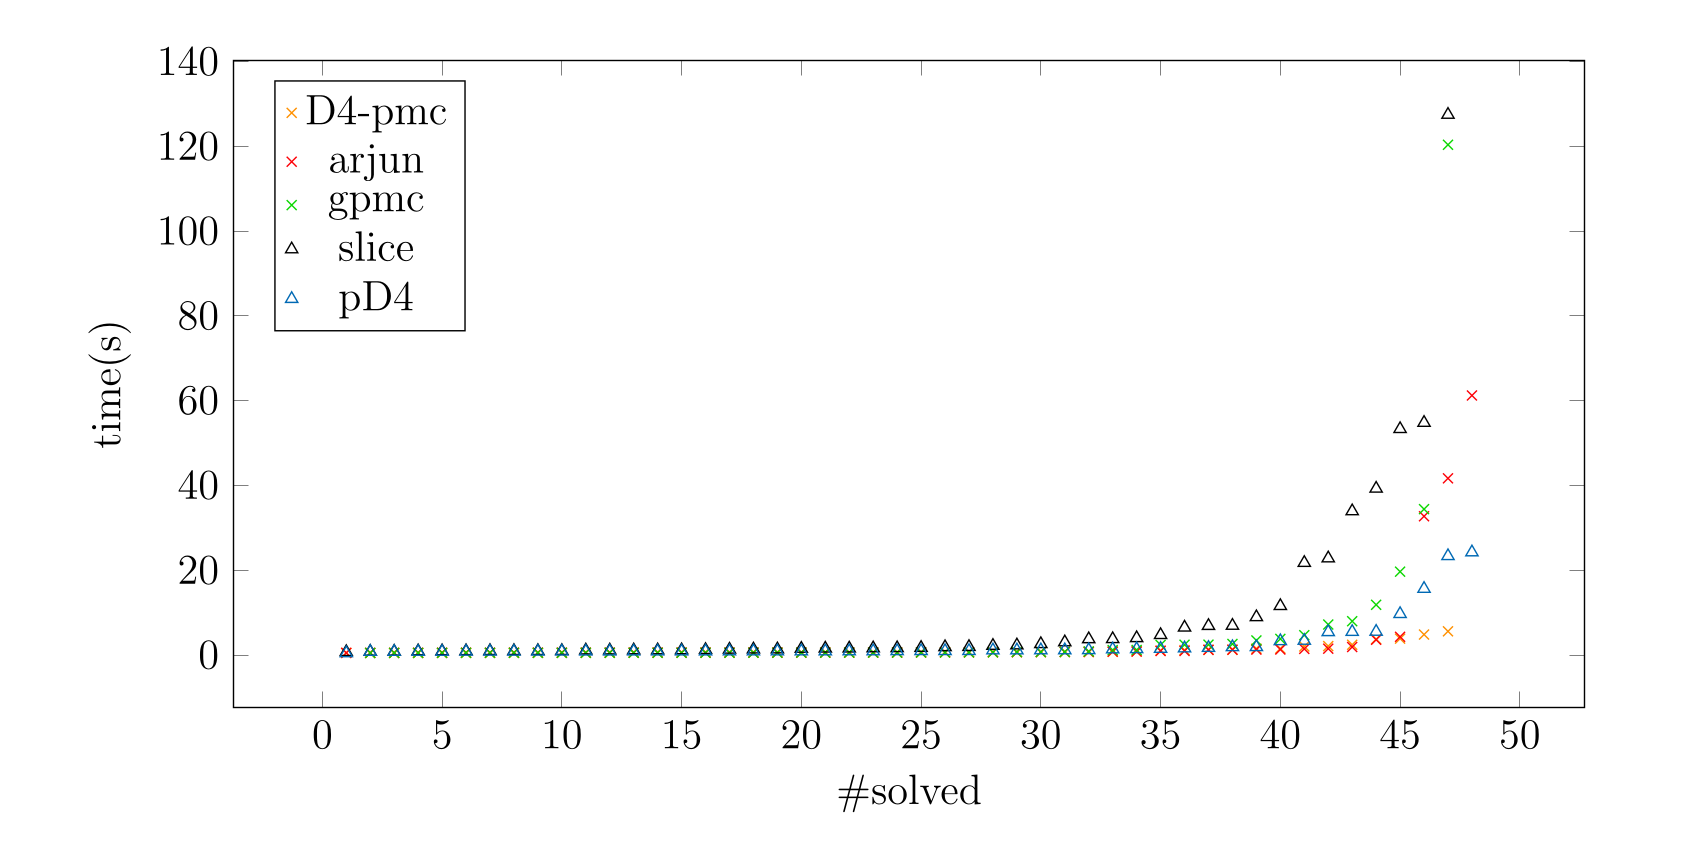
\includegraphics[width=12cm]{exp1.png}
\end{frame}
\begin{frame}{Experiment2: Generated Projection}
    \centering
    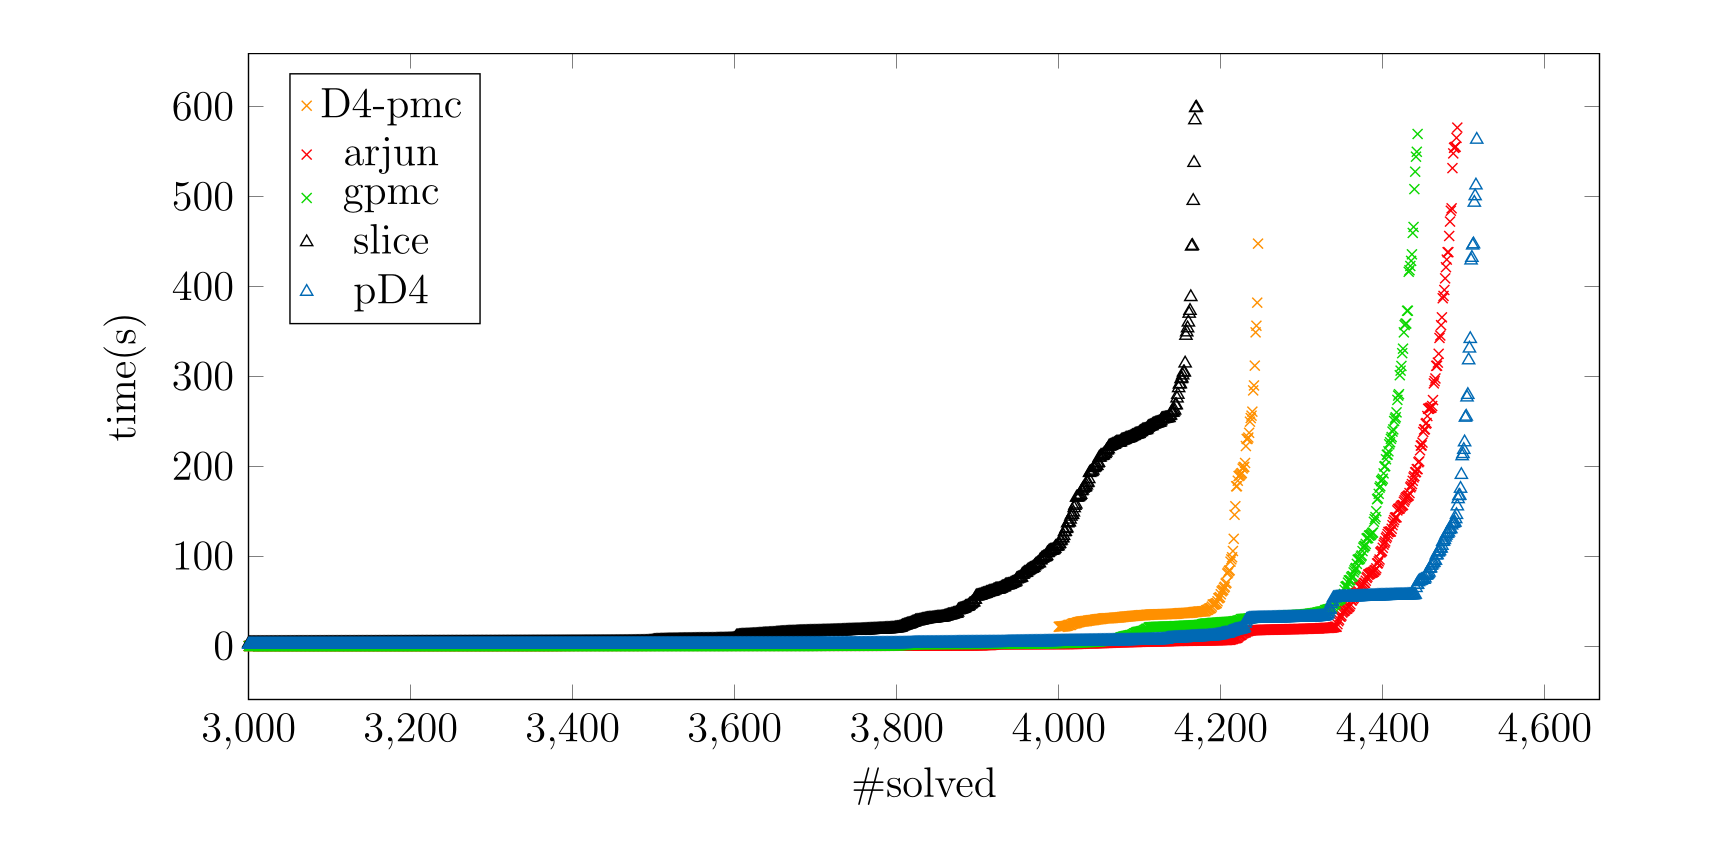
\includegraphics[width=12cm]{exp2.png}
\end{frame}
\begin{frame}{Experiment2: Generated Projection}
    \centering
    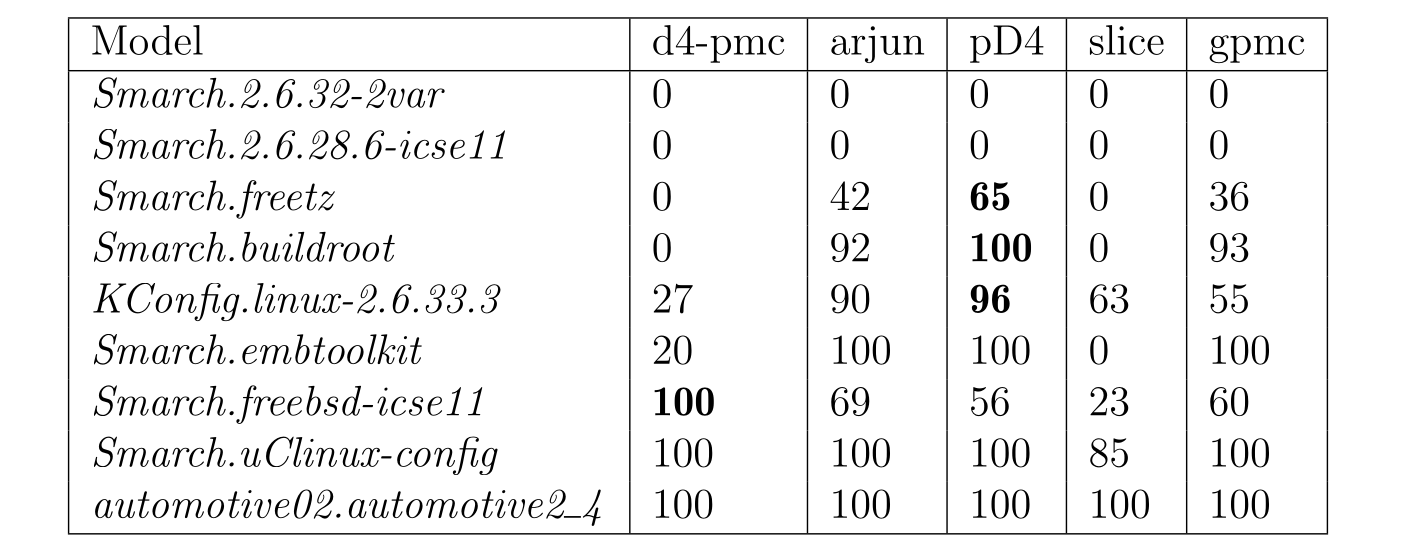
\includegraphics[width=12cm]{exp2-table.png}
\end{frame}
\begin{frame}{Experiment3: MC2022}
    \centering
    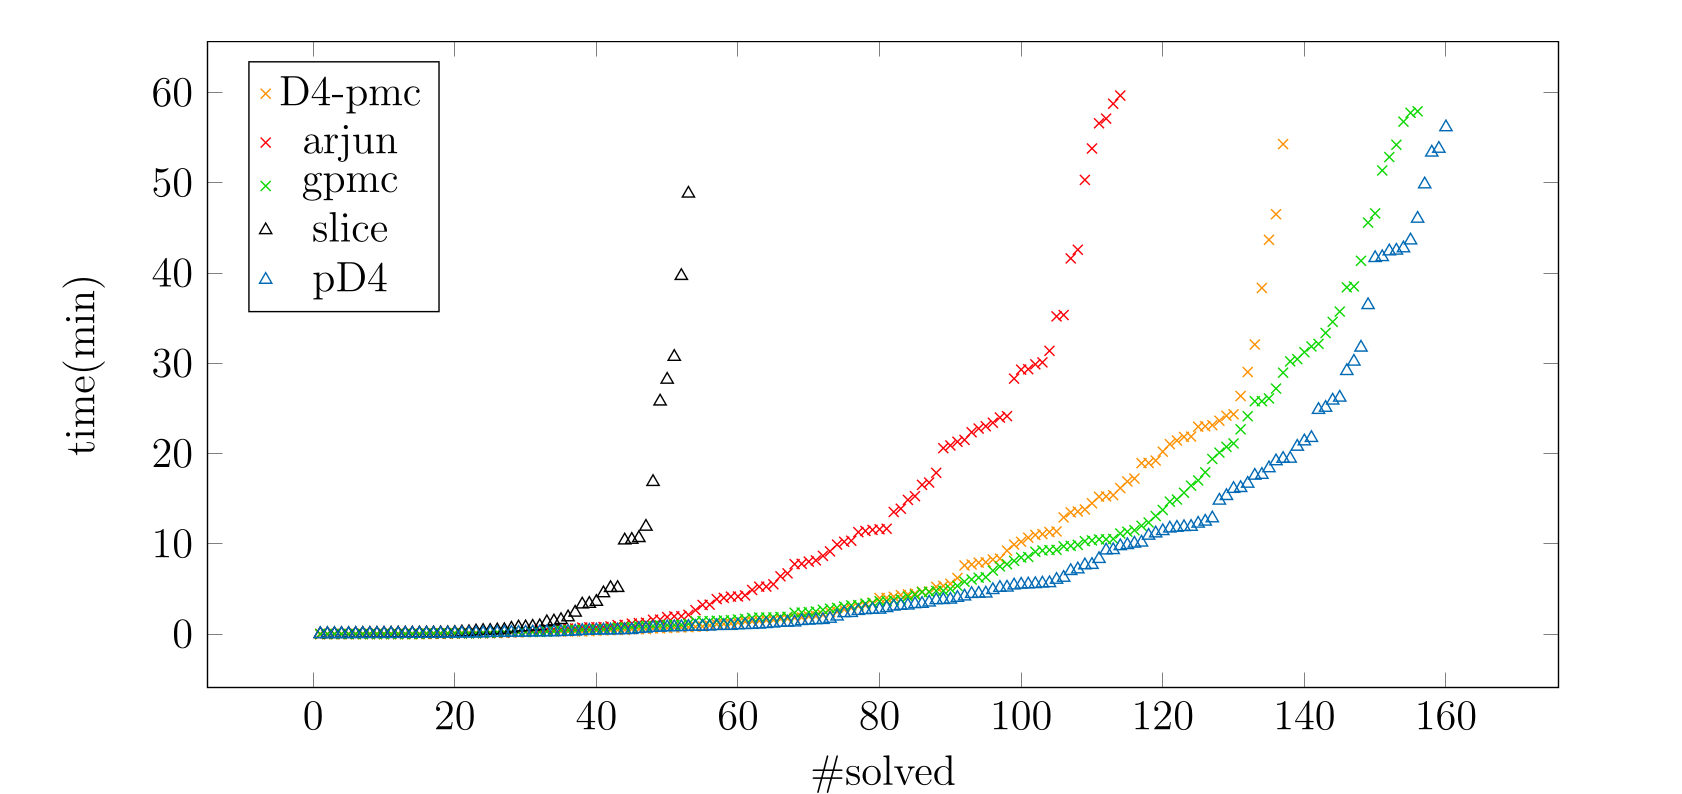
\includegraphics[width=12cm]{exp3.png}
\end{frame}

\begin{frame}{Recap and Feature Work}
    \begin{tikzpicture}[remember picture,overlay]
        \node[xshift=-4cm,yshift=-3cm,visible on = <5->] at (current page.north east) {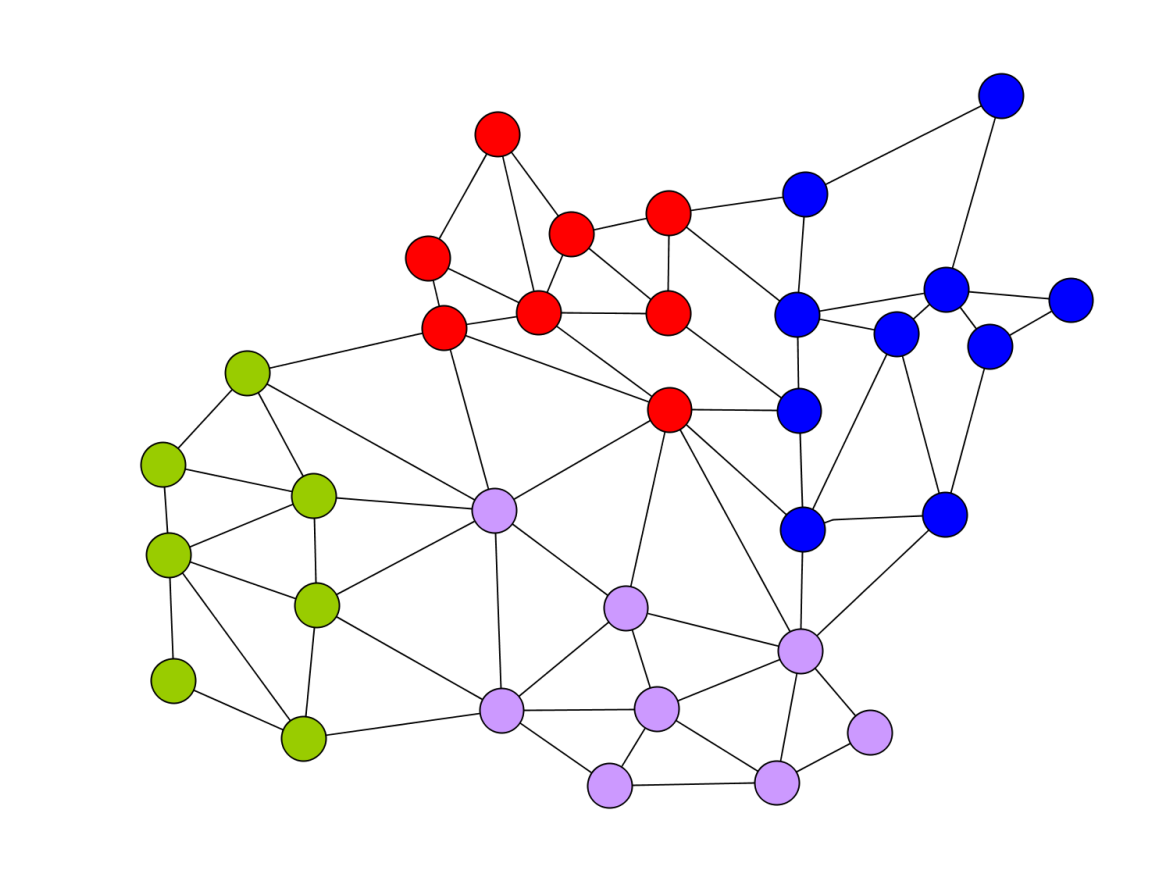
\includegraphics[width=6cm]{hyp2.png}};
        \node[xshift=-3cm,yshift=-7cm,visible on = <6->] at (current page.north east) {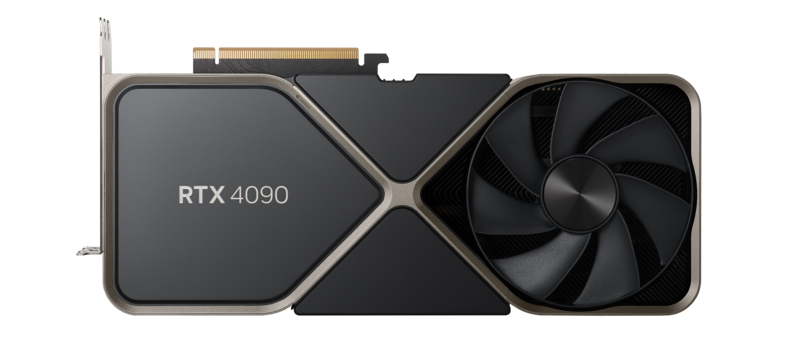
\includegraphics[width=4cm]{rtx.png}};
        \node[xshift=-6cm,yshift=-7cm,visible on = <6->] at (current page.north east) {
\includegraphics[width=2cm]{thread.png}};
        
    \end{tikzpicture}
    \begin{block}{Recap}
        \begin{itemize}
            \item Combine slice and d-DNNF compilation\pause
            \item New heuristics for good performance\pause
            \item Compile hard feature models like linux under projection \pause
            \item Often comparable or smaller d-DNNF size
        \end{itemize}
    \end{block}\pause
    \begin{block}{Future Work}
        Lots of new possible heuristics...\\ \pause
        Hardware acceleration...\\ \pause
        More applications for projected output d-DNNF 
    \end{block}

\end{frame}
\begin{frame}{The End}
\end{frame}
\end{document}